\chapter{3D Object Representation}

This chapter contains the definitions of various three-dimensional object representations
that are commonly used in applications. A geometric query or a different operation involving the
object might be more effectively formulated with one representation than another.

\section{Overview}

The 3D object representations can be divided into two major categories

\begin{itemize}
\item \textbf{solid} - the object in this representation contains information about inner
propreties of the object such as density and elasticity. It is mostly used in software for
engineering simulations.

\item \textbf{surface} - this representation works only with the surface of the object
ignoring the properties of the volume itself. One of the advantages of this representation is
relatively simple visualisation. The surface description is entirely sufficient for graphical purposes.
\end{itemize}

\subsection{Voxel Map}

A \textbf{voxel} is a word made by joining '\textbf{Vo}lumetric' and 'Pi\textbf{xel}'. It represents
the value on regular grid that forms a voxel map. The simplest representation of a voxel map is
a normalized grid made of cube-shaped voxels with 0-1 values where 0 stands for the cube that is completely
outside of the object and 1 represents the case of crossing the surface or inclusion by the object.
\\
\\
Each voxel can contain various properties such as color, material physical properties or
in case of boundary voxels, a surface description. Some implementations provide information about
each corner of voxel separately in order to improve the accuracy.
As it can be deduced from the overview, this representation is perfect for the representation
of the solid objects.

\subsection{Implicit Surface}
An implicit surface\cite{Agin1972} is a surface defined implicitly by a function

\begin{equation}
\begin{split}
surface_{f(x,y,z)} =
  &\left\{\;
    \begin{split}
      \text{on surface if }f(x,y,z) = 0 \\ 
      \text{below surface if }f(x,y,z) < 0 \\
      \text{above surface if }f(x,y,z) > 0 \\
    \end{split}
  \right.
\end{split}
\end{equation}

\begin{figure}[H]
\centering
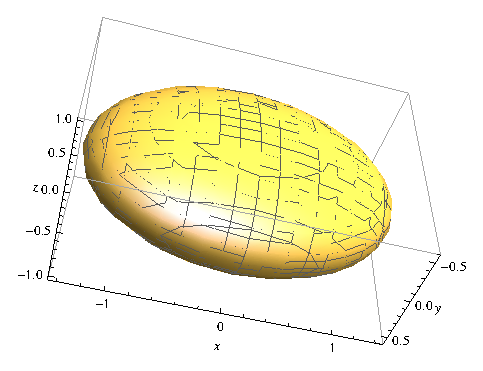
\includegraphics[scale=1]{../img/implicit_surface.eps}
\label{fig:implicit}
\caption{Implicit surface given by function $f(x,y,z) = \frac{1}{2}x^{2} + 3y^{2} + z^{2} = 1$}
\end{figure}
This representation has several advantages such as efficient checking whether a point is either
inside or outside and efficient search for an intersection with geometric primitives.


\subsection{Constructive Solid Geometry}

Known also as \emph{CSG tree}\cite{Zara2004}. This technique is used especially
in the engineering software. It allows
the user to construct objects using \emph{Boolean operators}. Objects created by using this
method can be used repeatedly in Boolean operators; the resulting object can be decomposed into a tree.
\\
\\
The leaves of the tree are typically the objects of the simple shape. However, the operators can be
theoretically applied on any objects. The set of supported primitives is given by a specific
software package.
\\
\\
Thanks to the tree structure, CSG objects come with some convenient properties. The nodes that
are higher in the tree hierarchy give us an approximation that can be used in various geometric
algorithms with no need to look for its descendants.

\subsection{Point Cloud}

A point cloud is a set of points in a three-dimensional coordinate system\cite{Zara2004}\cite{Agarwal2006}.
The set can form the surface
of an object or any other three dimensional figure. Every point is indepedent
from one another, with no information about its topology. They are often converted to polygon mesh
or triangle mesh models.

\subsection{Polygonal Mesh}

A polygonal mesh is a collection of vertices, edges and faces that defines the shape of the surface of
the object\cite{Zara2004}. Some special implementations do not contain faces. These implementations are
defined only by vertices and
edges. Moreover, some cases do not consider the topology and the object is a raw set of polygons.
Neverthless, a standard implementation is expected to contain a topology information about each vertex
and face.
\\
\\
Each face is defined by planar polygon, in special cases by \emph{convex polygon} or \emph{triagle}.
The polygonal mesh restricted to contain triangular faces only, is called \emph{triangle mesh}.
The main purpose of the restriction is the rendering simplification. In general case, face is defined
as the set of points that can contain a hole.
\\
\\
There are several techniques to represent a topology of the mesh. Each of them has its own advantages
that are reflected in an efficiency of data storage and querying the surrounding elements. Several
mesh representations are described in the next section.

\section{Polygonal Mesh}
\label{sec:polyg_mesh}
The collection can be represented in a variety of ways, the main purpose of the structure is to improve
the efficiency of the queries. On the other hand we face the limitations such as memory. In some
representations it is impossible to query the adjacent vertices of a vertex without iteration through
entire container of vertices or faces.

\subsection{Face-Vertex Mesh}
\label{sec:face-vertex}

The simplest representation that contains any information about topology of the polygonal
mesh. A mesh is represented by a container of vertices and the container of sets of vertices that
form faces\cite{Zara2004}. The face is represented by at least 3 vertices or more vertices that have to be
coplanar.\\

\begin{figure}[h]

\begin{minipage}[hb]{0.65\linewidth}
\centering
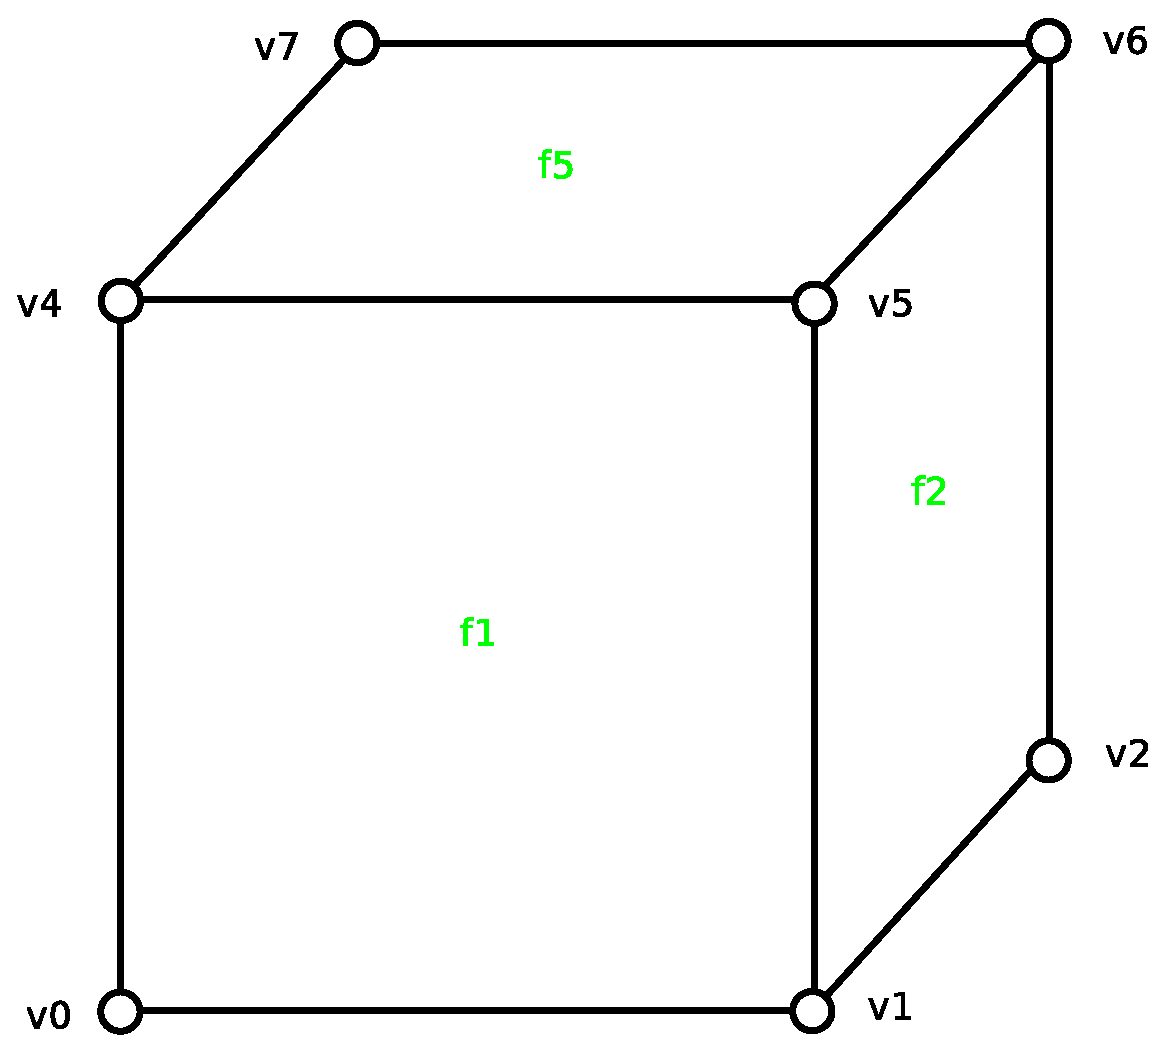
\includegraphics[width=0.6\linewidth]{../img/fv_rep_mesh.eps}
\label{fig:figure1}
\end{minipage}
\hspace{0.5cm}
\begin{minipage}[hb]{0.25\linewidth}
\centering
\begin{tabular}{|c|c|}
\hline
\textsf{v0 v1 v5 v4} & \textsf{f1}\\
\hline
\textsf{v1 v2 v6 v5} & \textsf{f2}\\
\hline
\textsf{v4 v5 v6 v7} & \textsf{f5}\\
\hline
\end{tabular}
\label{fig:fv_mesh}
\end{minipage}

\caption{face-vertex mesh representation}
\end{figure}

The set that forms the faces must be ordered. The preceding and following vertex in order must be 
adjacent to
the vertex. If the structure is not extended by face-normal-attribute, the vertices have to be in 
clockwise/counter-clockwise order from the view of face normal. Whether the order is clockwise or counter-clockwise
depends on the implementation of the mesh.

\subsection{Winged-Edge mesh}

The representation described above contains no direct information about adjacency of faces. 
In order to determine the adjacency of any two faces or vertices in constant complexity, we
can build a structure that requires an extra storage. The winged edge structure\cite{Baumgart1972}
provides information
capable of determining edges that belong to a vertex. It also provides information which allows us
to determine the surrounding edges from the given face;
in case of a triangle mesh, it returns the triplet of edges.
Finally, the structure is named \emph{winged-edge} because of its
capabilty to get a face pair (wings) from
a given edge.

\begin{figure}[!htbp]
\label{fig:winged_edge_mesh}

\begin{minipage}[!htbp]{0.65\linewidth}
\centering
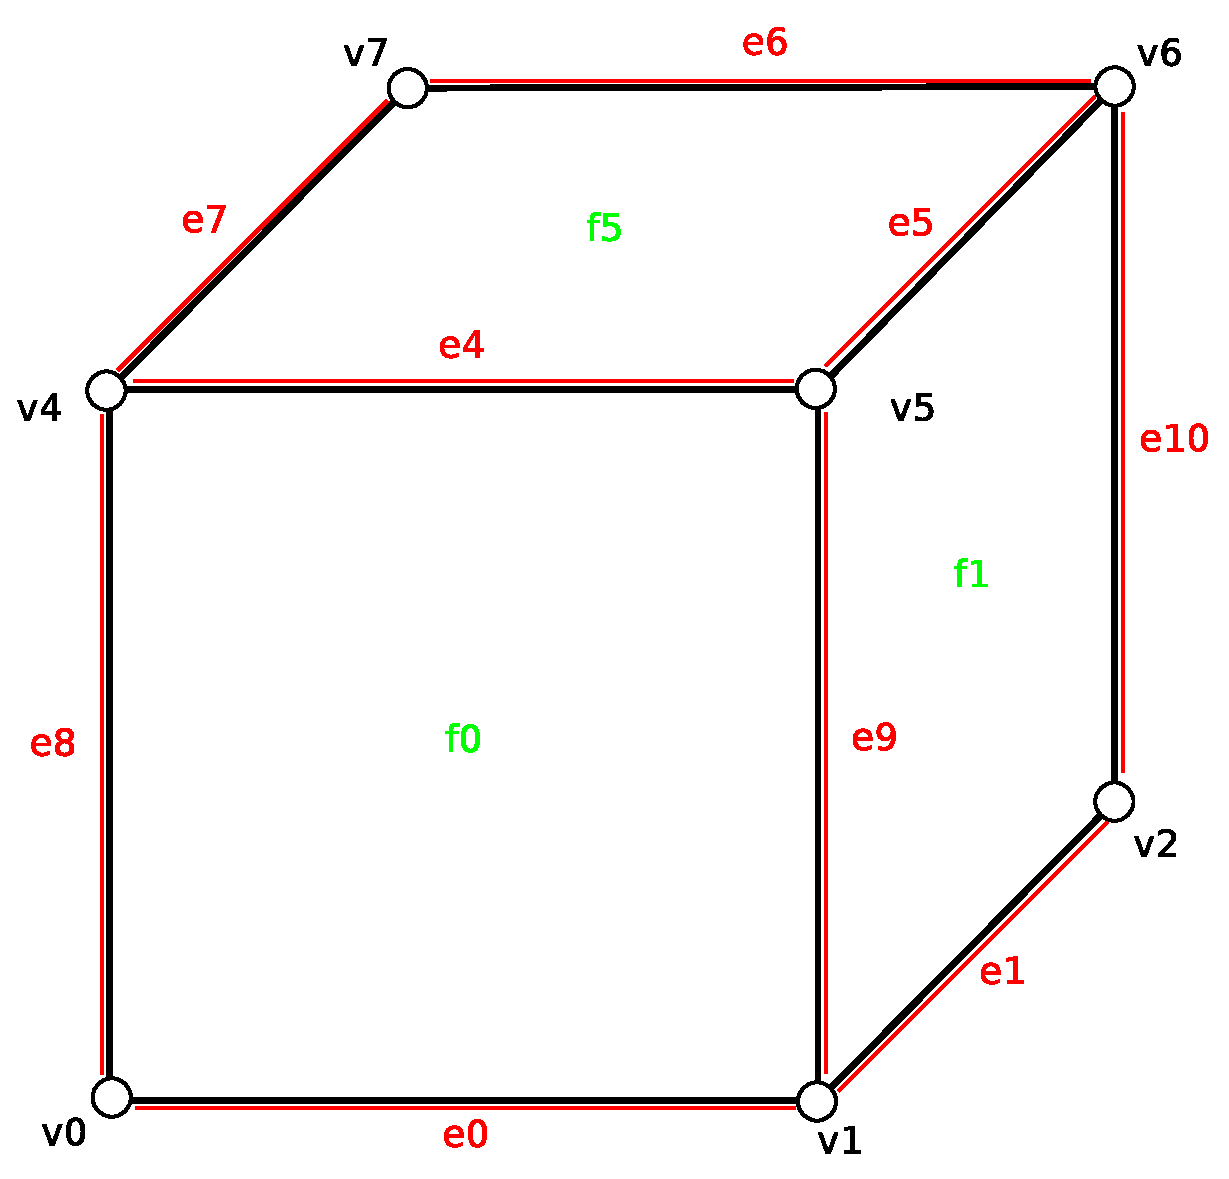
\includegraphics[width=0.6\linewidth]{../img/we_rep_mesh.eps}
\label{fig:figure1}
\end{minipage}
\hspace{0.5cm}
\begin{minipage}[!htbp]{0.25\linewidth}
\centering

\emph{Face list}
\vspace{1mm}

\begin{tabular}{|c|c|}
\hline
\textsf{f0} & \textsf{e0 e9 e4 e8}\\
\hline
\textsf{f1} & \textsf{e1 e10 e5 e9}\\
\hline
\textsf{f5} & \textsf{e4 e5 e6 e7}\\
\hline
\end{tabular}

\vspace{10mm}
\emph{Edge list}
\vspace{1mm}

\begin{tabular}{|c|c|c|}
\hline
\textsf{e0} & \textsf{f0 f4} & \textsf{v0 v1}\\
\hline
\textsf{e1} & \textsf{f1 f4} & \textsf{v1 v2}\\
\hline
\textsf{e4} & \textsf{f0 f5} & \textsf{v4 v5}\\
\hline
\textsf{e5} & \textsf{f1 f5} & \textsf{v5 v6}\\
\hline
\textsf{e6} & \textsf{f2 f5} & \textsf{v6 v7}\\
\hline
\textsf{e7} & \textsf{f3 f5} & \textsf{v7 v8}\\
\hline
\textsf{e8} & \textsf{f0 f3} & \textsf{v4 v0}\\
\hline
\textsf{e9} & \textsf{f1 f0} & \textsf{v5 v1}\\
\hline
\textsf{e10} & \textsf{f2 f1} & \textsf{v6 v2}\\
\hline
\end{tabular}

\label{fig:we_mesh}
\end{minipage}

\caption{Winged-edge mesh}
\end{figure}

%On the example shown above there are occured several uncertainities.
Several uncertainities occured in the above-mentioned examples.

\begin{itemize}
\item Let us take edge \textsf{e9}. In the pair of faces, which of faces \textsf{f0} and 
\textsf{f1} should be considered as the \emph{first} and which as the \emph{second}?

\item Which of vertices \textsf{v1} and \textsf{v5} should be considered as 
the \emph{first} and which as the \emph{second} in the pair that forms the edge \textsf{e9}?
\end{itemize}

One of possible solutions is to split the edge element into two \emph{half-edges}.
The structure using, or rather based on this representation, is described in the next
paragraph.

\subsection{Half-Edge mesh}

The half-edge data structure is the structure capable of maintaining the incidence
information of vertices, edges and faces\cite{Botsch2006}. Each edge is decomposed in two half-edges
with opposite orientations.
\\

The structure contains the set of following information
\begin{itemize}
\item a vertex that is the half-edge pointing to
\item a face that the half-edge belongs to
\item the next half-edge in order that forms a face that half-edge belongs to
\item (optional) the previous half-edge in the same order
\item opposite half-edge
\end{itemize}

\begin{figure}[h]

\begin{minipage}[hb]{0.65\linewidth}
\centering
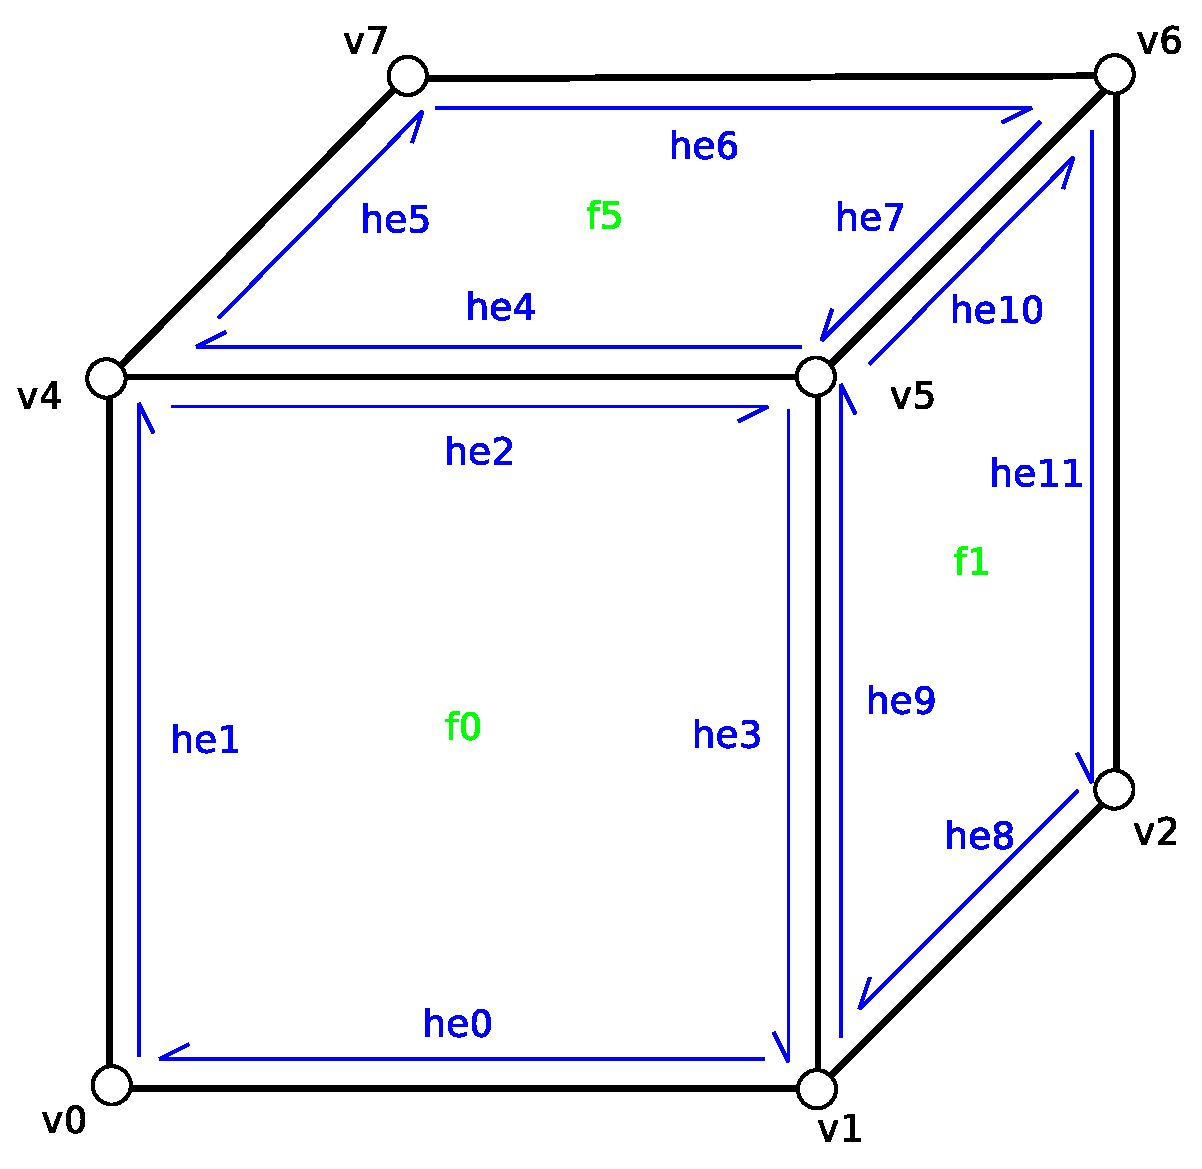
\includegraphics[width=0.6\linewidth]{../img/he_rep_mesh.eps}
\label{fig:figure1}
\end{minipage}
\hspace{0.5cm}
\begin{minipage}[hb]{0.25\linewidth}
\centering
\emph{Half-edge list}
\vspace{1mm}

\begin{tabular}{|c|c|c|c|}
\hline
\textsf{he0} & \textsf{f0} & \textsf{v0} & \textsf{he1}\\
\hline
\textsf{he1} & \textsf{f0} & \textsf{v4} & \textsf{he2}\\
\hline
\textsf{he2} & \textsf{f0} & \textsf{v5} & \textsf{he3}\\
\hline
\textsf{he3} & \textsf{f0} & \textsf{v1} & \textsf{he0}\\
\hline

\hline
\textsf{he8} & \textsf{f1} & \textsf{v1} & \textsf{he9}\\
\hline
\textsf{he9} & \textsf{f1} & \textsf{v5} & \textsf{he10}\\
\hline
\textsf{he10} & \textsf{f1} & \textsf{v6} & \textsf{he11}\\
\hline
\textsf{he11} & \textsf{f1} & \textsf{v2} & \textsf{he8}\\
\hline

\hline
\textsf{he4} & \textsf{f5} & \textsf{v4} & \textsf{he5}\\
\hline
\textsf{he5} & \textsf{f5} & \textsf{v7} & \textsf{he6}\\
\hline
\textsf{he6} & \textsf{f5} & \textsf{v6} & \textsf{he7}\\
\hline
\textsf{he7} & \textsf{f5} & \textsf{v5} & \textsf{he4}\\
\hline
\end{tabular}
\label{fig:he_mesh}
\end{minipage}

\caption{Half-edge mesh representation}

\end{figure}
